\section{Results}
\label{sec:results}

% Rows are generated by experiments/analysis/paper_results.py (<group>_paper.tex).
\newcommand{\resulttable}[3]{%
\begin{table}[t]
\centering
\caption{#2 Mean$_{\pm\text{std}}$ over three seeds; best mean in bold. FPR in \%.}
\label{#3}
\footnotesize
\setlength{\tabcolsep}{3pt}
\IfFileExists{\results{#1}}{%
\CatchFileDef{\resultrows}{\results{#1}}{}% \input is not usable inside a tabular
\resizebox{\columnwidth}{!}{%
\begin{tabular}{@{}lcccccc@{}}
\toprule
Method & OW-F1 & AUT & Det-F1 & FPR & U-AUROC & Forget.\\
\midrule
\resultrows
\bottomrule
\end{tabular}}}{\TBD{\detokenize{#1} not generated yet}}
\end{table}}

\subsection{Main comparison}
\resulttable{CIC17_main_b010_paper.tex}{CIC-IDS2017, label budget 10\%, delay 1 window.}{tab:cic17}
\resulttable{IDS18_main_b010_paper.tex}{CSE-CIC-IDS2018, label budget 10\%, delay 1 window.}{tab:ids18}
\resulttable{UNSW_main_b010_paper.tex}{UNSW-NB15 (four classes held out of training), label budget 10\%.}{tab:unsw}

\textbf{CIC-IDS2017} (\cref{tab:cic17}). \nova{} has the highest OW-F1 (0.768) and AUT (0.858), but its lead
over CBRS replay (0.756, 0.838) is within the bootstrap uncertainty (per-window difference $+2.0$ points, 95\% CI
$[-0.5, +4.3]$). It is significantly ahead of every other method (by 6.8 to 22.8 points). CBRS detects slightly
more attacks (detection F1 0.861 against 0.854), but \nova{} flags significantly fewer benign flows (4.5\% against
2.8\% pooled; per-window difference $-4.0$, CI $[-8.8, -0.5]$): it sends 38\% fewer benign flows to the analyst.

\begin{figure}[t]
\centering
\IfFileExists{\results{fig_ow_f1_over_time_UNSW_col.pdf}}{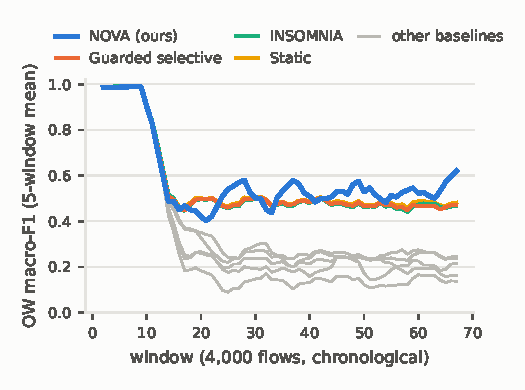
\includegraphics[width=\columnwidth]{fig_ow_f1_over_time_UNSW_col.pdf}}{\TBD{figure}}
\caption{OW macro-F1 per window on UNSW-NB15 (mean of three seeds, 5-window moving average). Replay-based
baselines (grey) fall below the static model.}
\label{fig:time-unsw}
\end{figure}

\textbf{CSE-CIC-IDS2018} (\cref{tab:ids18}). \nova{} and CBRS replay tie on OW-F1 (0.722) and AUT (0.869;
difference CI $[-1.9, +1.9]$). \nova{} has the higher detection F1 (0.815 against 0.788), a significantly lower
false-positive rate (3.1\% against 4.8\%; CI $[-6.9, -0.4]$) and five times less forgetting (0.007 against 0.034).

\textbf{UNSW-NB15} (\cref{tab:unsw}, \cref{fig:time-unsw}). Most adaptive methods end \emph{below} the static
model (0.499); CBRS replay reaches 0.327. They learn Exploits and Fuzzers, but every later flow of these classes is
rejected as \unk{}: the thresholds were calibrated on January traffic, and February flows of the same classes lie
outside them. \nova{} recalibrates learned classes on its calibration store and reaches 0.509 OW-F1 and 0.595
AUT, significantly ahead of every replay-based method ($+19.5$ to $+29.3$ points) and level with the static model
($+2.6$, CI $[-0.1, +4.8]$), with the highest detection F1 (0.860) and lowest false-positive rate (6.6\% against
7.6--19.0\%). On the classes the model knows, \nova{} reaches a macro-F1 of 0.510 against at most 0.165 for any
other method. Without the calibration store, \nova{} drops to 0.418 and zero F1 on Exploits and Fuzzers
(\cref{tab:ablation}), confirming the mechanism.

INSOMNIA's self-training has the highest false-positive rate on both CIC datasets (12.4\%, 25.7\%):
pseudo-label errors on unseen classes are fed back into training.

\Cref{fig:time-cic} shows where the methods differ on CIC-IDS2017. Every method drops when a new attack class
starts. CBRS replay recovers faster from the first DoS attacks (windows 8--12), \nova{} from most later ones,
most visibly in the last ten windows.

\begin{figure*}[t]
\centering
\IfFileExists{\results{fig_ow_f1_over_time_CIC17.pdf}}{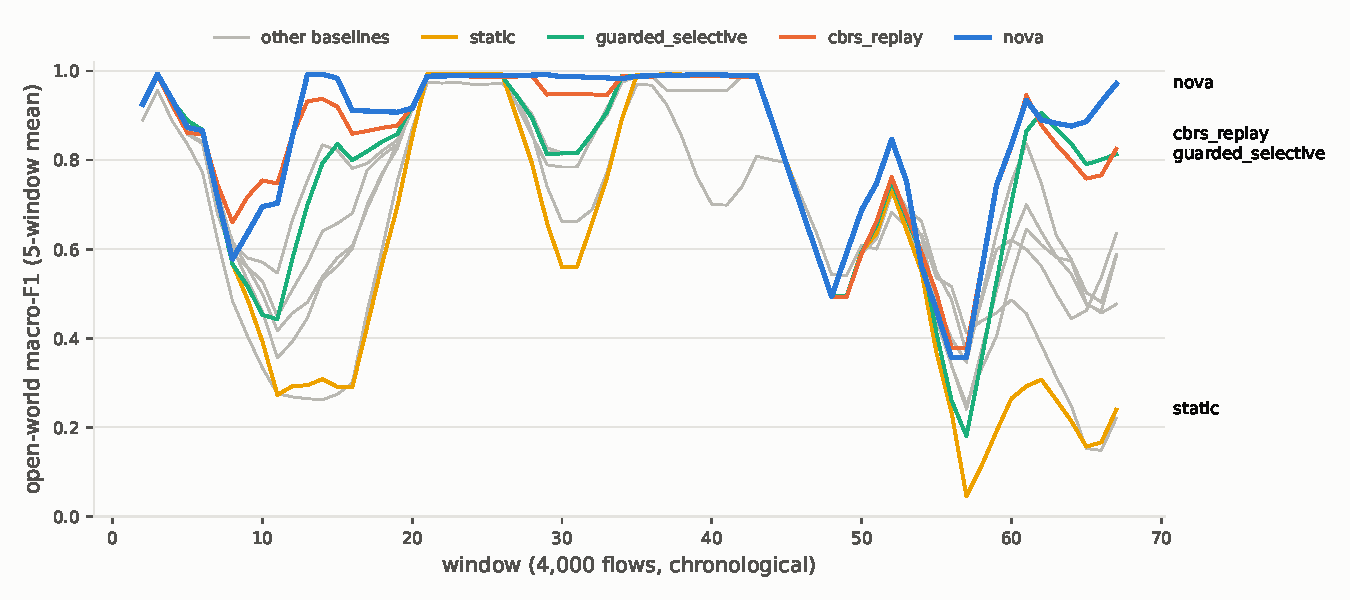
\includegraphics[width=0.8\textwidth]{fig_ow_f1_over_time_CIC17.pdf}}{\TBD{figure}}
\caption{OW macro-F1 per window on CIC-IDS2017 (mean of three seeds, 5-window moving average). \nova{}, the two
strongest baselines and the static model in colour, the other baselines in grey.}
\label{fig:time-cic}
\end{figure*}


\subsection{Label budget}
With 1\% of each window labelled (\cref{tab:budget}), \nova{} leads CBRS replay by 9.0 points on CIC-IDS2017
(per-window CI $[+1.4, +11.6]$) and by 3.4 points on CSE-CIC-IDS2018 (CI $[-0.2, +5.0]$, not significant). On
UNSW-NB15 it trails periodic retraining (0.469 against 0.504). With 40 labels per window, periodic retraining never
collects enough labels of the held-out classes to learn them, so it keeps rejecting them as \unk{}, which the
metric credits in full. Its macro-F1 on the classes the model knows is only 0.154, against 0.383 for \nova{}, which
names 64\% of known attack flows correctly against 7\%. \nova{} learns DoS and Reconnaissance, which overlap with
Exploits, and loses the \unk{} credit; open-world macro-F1 alone cannot separate ``never learned'' from ``learned
imperfectly''. \nova{} also halves the false-positive rate (9.7\% against $\geq$15.7\%).

\begin{table}[t]
\centering
\caption{Label budget 1\%: OW macro-F1 and FPR (\%), mean over three seeds; best per column in bold.}
\label{tab:budget}
\footnotesize
\setlength{\tabcolsep}{3pt}
\IfFileExists{\results{budget_b001_paper.tex}}{%
\CatchFileDef{\budgetrows}{\results{budget_b001_paper.tex}}{}%
\resizebox{\columnwidth}{!}{%
\begin{tabular}{@{}lcccccc@{}}
\toprule
\budgetrows
\bottomrule
\end{tabular}}}{\TBD{budget table not generated yet}}
\end{table}

\subsection{Ablation and detector}
\begin{table}[t]
\centering
\caption{Ablation (budget 10\%): OW-F1 (change in points) and FPR (\%) with one component removed. Mean over
three seeds; full \nova{} over the same seeds. Only CIC-IDS2017 was used for design.}
\label{tab:ablation}
\footnotesize
\setlength{\tabcolsep}{2pt}
\IfFileExists{\results{ablation_all_paper.tex}}{%
\CatchFileDef{\ablrows}{\results{ablation_all_paper.tex}}{}%
\resizebox{\columnwidth}{!}{%
\begin{tabular}{@{}lcccccc@{}}
\toprule
 & \multicolumn{2}{c}{CIC-IDS2017} & \multicolumn{2}{c}{CSE-CIC-IDS2018} & \multicolumn{2}{c}{UNSW-NB15} \\
Variant & OW-F1 & FPR & OW-F1 & FPR & OW-F1 & FPR \\
\midrule
\ablrows
\bottomrule
\end{tabular}}}{\TBD{ablation table not generated yet}}
\end{table}

On CIC-IDS2017 every removal lowers OW-F1 (\cref{tab:ablation}), most for the guard ($-5.6$, in every seed). The
loss is concentrated in XSS and Bot: without the guard, models that name XSS flows Brute Force are deployed, whereas
with it XSS stays \unk{} and receives full open-world credit. Per window, no single removal is significant on
CIC-IDS2017. On UNSW-NB15 the guard and the calibration store are essential ($-22.1$, $-9.1$); both variants lose
Exploits and Fuzzers. On CSE-CIC-IDS2018 the stream-level changes have inconsistent signs across seeds, because four
of its classes have only 2 to 33 flows. Per window, only the query and propagation help significantly there
(block-bootstrap CIs $[-3.1, -0.3]$ and $[-3.6, -0.5]$). Replacing the class-conditional $k$-NN detector by
distance to the nearest class centroid lowers OW-F1 from 0.768 to 0.712 for \nova{} and from 0.311 to 0.178 for
the static model, which then labels almost every attack benign: one centroid cannot follow multi-modal benign
traffic.

\textbf{Neural classifier.} With an MLP instead of gradient boosting on CIC-IDS2017, \nova{} keeps the lowest
false-positive rate (3.3\% against 4.7\%), the higher detection F1 and an equal AUT, but its OW-F1 is lower than
CBRS replay's (0.622 against 0.711), mainly on two short-lived web attacks. We do not claim that its accuracy
advantage carries over to neural classifiers.
